\chapter{Từ thông - Hiện tượng cảm ứng điện từ}
\section{Lý thuyết trọng tâm}
\subsection{Từ thông}
\subsubsection{Biểu thức tính từ thông}
\begin{center}
	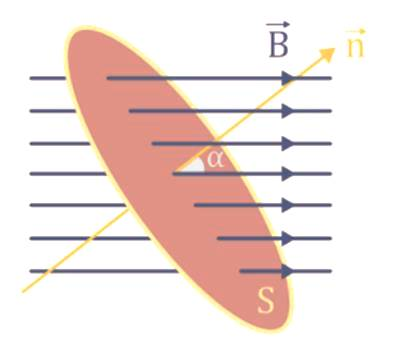
\includegraphics[scale=0.6]{../figs/VN11-PH-29-L-020-1-h63.jpg}
\end{center}
Từ thông $\Phi$ có biểu thức:
\begin{equation}
\Phi=BS\cos \alpha,
\end{equation}
với $\alpha$ là góc hợp bởi $\vec{B}$ và $\vec{n}$, trong đó,
\begin{itemize}
	\item $\vec{n}$ là véctơ pháp tuyến dương của mặt $S$,
	\item $B$ là cảm ứng từ, 
	\item $S$ là diện tích của mặt phẳng tạo bởi vòng dây,
	\item $\Phi$ là từ thông qua mặt $S$. 
\end{itemize}

Đơn vị của từ thông là vêbe (Wb). Trong công thức trên, nếu $S=1\ \text{m}^2, \ B=1\ \text{T}$ thì $\Phi=1\ \text{Wb}$.

Trường hợp khung dây có $N$ vòng dây thì

 \begin{equation}
 \Phi=NBS\cos \alpha.
 \end{equation}

\subsubsection{Giá trị của từ thông}
Từ thông $\Phi$ là \textit{đại lượng đại số}.
\begin{itemize}
\item $\Phi >0$ khi $0<\alpha <90^\circ$,
\item $\Phi =0$ khi $\alpha =90^\circ$,
\item $\Phi <0$ khi $90^\circ<\alpha <180^\circ$.
\end{itemize}


\subsubsection{Các cách làm biến thiên từ thông}
Có 3 cách làm biến thiên từ thông:
\begin{itemize}
	\item Thay đổi $B$, tức là thay đổi số đường sức từ đi qua mặt $S$.
	\item Thay đổi $S$, tức là thay đổi diện tích vòng dây.
	\item Thay đổi góc $\alpha$, tức là thay đổi góc hợp bởi véctơ pháp tuyến của vòng dây với các đường sức từ.
\end{itemize}
\subsection{Hiện tượng cảm ứng điện từ}
\subsubsection{Dòng điện cảm ứng}
Mỗi khi từ thông qua một mạch kín biến thiên thì trong mạch xuất hiện một dòng điện, gọi là dòng điện cảm ứng.
\subsubsection{Hiện tượng cảm ứng điện từ}
Hiện tượng xuất hiện dòng điện cảm ứng trong mạch được gọi là hiện tượng cảm ứng điện từ.

Hiện tượng cảm ứng điện từ chỉ tồn tại trong khoảng thời gian từ thông qua mạch kín biến thiên.



\section{Bài tập}
\begin{dang}{Biểu thức từ thông}
\end{dang}

\textbf{Phương pháp giải}

Sử dụng biểu thức tính từ thông:
\begin{equation}
\Phi=BS\cos \alpha,
\end{equation}
với $\alpha$ là góc hợp bởi $\vec{B}$ và $\vec{n}$

\luuy{Khi đề bài cho góc $\beta$ là góc hợp bởi véctơ cảm ứng từ và mặt phẳng khung dây thì ta phải tính góc $\alpha$ tạo bởi véctơ pháp tuyến và mặt phẳng khung dây bằng cách $\alpha=90^\circ -\beta$.}

{\viduii{2}{
	
Một khung dây có các tiết diện là hình tròn, bán kính khung dây là 20 cm, khung dây được đặt vuông góc với các đường sức từ của một từ trường đều có $B=2\cdot 10^-5\ \text{T}$.   Hãy xác định giá trị của từ thông xuyên qua khung dây nói trên?
\begin{mcq}(2)
	\item $0\ \text{Wb}$.
	\item $\text{2,51}\cdot 20^{-6}\ \text{Wb}$.
	\item $\text{5,02}\cdot 20^{-6}\ \text{Wb}$.
	\item $\text{1,26}\cdot 20^{-6}\ \text{Wb}$.
\end{mcq}}{
\begin{center}
	\textbf{Hướng dẫn giải:}
\end{center}

Tiết diện của khung là $S=\pi R^2=\text{0,04}\pi \text{m}^2$.

Do khung dây được đặt vuông góc với các đường sức từ nên $\alpha=0$.

Từ thông xuyên qua khung dây là $\Phi=BS\cos \alpha=\text{2,51}\cdot 10^{-6}\ \text{Wb}$.
	
\textbf{Đáp án: B.}}
}

{\viduii{2}{
	
Một khung dây hình vuông có cạnh dài 5 cm, đặt trong từ trường đều cảm ứng từ $B=5\cdot 10^{-2}\ \text{T}$, khung dây tạo với các đường sức một góc $30^\circ$. Hãy tính từ thông xuyên qua khung dây?
\begin{mcq}(2)
	\item $\text{6,25}\cdot 20^{-5}\ \text{Wb}$.
	\item $\text{7,25}\cdot 20^{-5}\ \text{Wb}$.
	\item $\text{10,08}\cdot 20^{-5}\ \text{Wb}$.
	\item $\text{1,25}\cdot 20^{-5}\ \text{Wb}$.
	
\end{mcq}}
{\begin{center}
	\textbf{Hướng dẫn giải:}
\end{center}
	
Mặt phẳng khung dây làm thành với $\vec{B}$ góc $30^\circ$ nên góc giữa $\vec{B}$ và pháp tuyến $\vec{n}$ là $\alpha=90^\circ -30^\circ=60^\circ$.

Diện tích hình vuông là $S=a^2=\text{2,5}\cdot 10^{-3}\ \text{m}^2$.

Từ thông xuyên qua khung dây là $\Phi=BS\cos \alpha=\text{6,25}\cdot 10^{-5}\ \text{Wb}$.


\textbf{Đáp án: A.}
}}

{\viduii{2}{
	
	Một hình vuông có cạnh là 5 cm, đặt trong từ trường đều có $B=\dfrac{8\sqrt{3}}{3}\cdot 10^{-4}\ \text{T}$, từ thông xuyên qua khung dây là $10^{-6}\ \text{Wb}$. Hãy xác định góc tạo bởi mặt phẳng khung dây và véctơ cảm ứng từ xuyên qua khung dây?
\begin{mcq}(4)
		\item $90^\circ$.
		\item $30^\circ$.
		\item $60^\circ$.
		\item $45^\circ$.
		
	\end{mcq}}{
\begin{center}
		{\textbf{Hướng dẫn giải:}}
\end{center}
		
		Từ thông xuyên qua khung dây là $\Phi=BS\cos \alpha \Rightarrow \cos \alpha= \dfrac{\Phi}{BS}=\dfrac{\sqrt{3}}{2}\Rightarrow \alpha= 30^\circ$.
		
		Góc giữa $\vec{B}$ và pháp tuyến $\vec{n}$ là $\alpha=30^\circ$ nên mặt phẳng khung dây làm thành với $\vec{B}$ góc $\beta= 90^\circ - 30^\circ=60^\circ$.  
		
	\textbf{	Đáp án: C.}}
	}

\begin{dang}{Hiện tượng cảm ứng điện từ}
\end{dang}

\textbf{Phương pháp giải}

Mỗi khi từ thông qua một mạch kín biến thiên thì trong mạch xuất hiện một dòng điện, gọi là dòng điện cảm ứng.

Hiện tượng xuất hiện dòng điện cảm ứng trong mạch được gọi là hiện tượng cảm ứng điện từ.

Hiện tượng cảm ứng điện từ chỉ tồn tại trong khoảng thời gian từ thông qua mạch kín biến thiên.

\luuy{Muốn xảy ra hiện tượng cảm ứng điện từ thì từ thông qua mạch phải biến thiên. Do đó, ta cần lưu ý 3 cách làm biến thiên từ thông là 
	\begin{itemize}
		\item thay đổi $B$, tức là thay đổi số đường sức từ đi qua mặt $S$.
		\item thay đổi $S$, tức là thay đổi diện tích vòng dây.
		\item thay đổi góc $\alpha$, tức là thay đổi góc hợp bởi véctơ pháp tuyến của vòng dây với các đường sức từ.
\end{itemize}}

{\viduii{1}{
	
	Một vòng dây dẫn được đặt trong một từ trường đều, sao cho mặt phẳng của vòng dây vuông góc với đường cảm ứng. Hiện tượng cảm ứng điện từ xảy ra khi
	\begin{mcq}
		\item nó bị làm cho biến dạng.
		\item nó được quay xung quanh pháp tuyến của nó.
		\item nó được dịch chuyển tịnh tiến.
		\item nó được quay xung quanh một trục trùng với đường cảm ứng từ.
	\end{mcq}}{
	\begin{center}
		\textbf{Hướng dẫn giải:}
	\end{center}
	
	Hiện tượng cảm ứng điện từ xảy ra khi từ thông $\Phi$ thay đổi. 
	
	Ở câu A, vòng dây biến dạng tức là diện tích $S$ thay đổi.
	
	Còn ở các câu B, C, D thì từ thông $\Phi$ không thay đổi nên không xảy ra hiện tượng cảm ứng điện từ.
	
\textbf{	Đáp án: A.}
}}

{\viduii{1}{
	
	Trong một vùng không gian rộng có một từ trường đều. Tịnh tiến một khung dây phẳng, kín theo những cách sau đây: 
	\begin{enumerate}[label=\Roman*]
		\item Mặt phẳng khung vuông góc với các đường cảm ứng.  
		\item Mặt phẳng khung song song với các đường cảm ứng.  
		\item Mặt phẳng khung hợp với các đường cảm ứng một góc $\alpha$.
	\end{enumerate}
	Trường hợp nào xuất hiện dòng điện cảm ứng trong khung?
		\begin{mcq}(2)
		\item Trường hợp I.
		\item Trường hợp II.
		\item Trường hợp III.
		\item Không có trường hợp nào.
	\end{mcq}}{
\begin{center}
		\textbf{Hướng dẫn giải:}
\end{center}
	
	Hiện tượng cảm ứng điện từ xảy ra khi từ thông $\Phi$ thay đổi. Nhưng trong cả 3 trường hợp I, II, III thì từ thông $\Phi$ không thay đổi nên không có trường hợp nào xuất hiện dòng cảm ứng.
	
\textbf{	Đáp án: D.}}
}

{\viduii{1}{
	
	Khung dây kín đặt vuông góc với các đường sức của một từ trường đều, rộng. Trong trường hợp nào sau đây, hiện tượng cảm ứng điện từ \textbf{không xảy ra}?
	\begin{mcq}
		\item Khung dây chuyển động tịnh tiến với tốc độ tăng dần.
		\item Khung dây quay quanh một đường kính của nó.
		\item Khung dây đứng yên nhưng bị bóp méo.
		\item Khung dây vừa chuyển động tịnh tiến, vừa bị bóp méo.
	\end{mcq}}{
\begin{center}
		\textbf{Hướng dẫn giải:}
\end{center}
	
	Khung dây chuyển động tịnh tiến thì góc hợp bởi $\vec{B}$ và véctơ pháp tuyến $\vec{n}$ của khung dây không đổi. Mà độ lớn cảm ứng từ $B$ và diện tích $S$ cũng không đổi nên từ thông không thay đổi.
	
\textbf{	Đáp án: A.}}
}



